\documentclass[a4paper, 12pt]{article}
\usepackage[utf8]{inputenc}
\usepackage[brazil]{babel}
\usepackage{amsmath}
\usepackage{cite}
\usepackage{graphicx}
\usepackage{color}
\usepackage{xcolor}
\usepackage{tikz}
\usepackage{hyperref}
\usepackage{xspace}
\hypersetup{
    colorlinks=true,
    linkcolor=black,
    citecolor=black,
    filecolor=black,
    urlcolor=black,
}
\newcommand{\tikzmark}[1]{\tikz[overlay, remember picture] \coordinate (#1);}

% Macros for proof-reading
\usepackage[normalem]{ulem} % for \sout
%\newcommand{\ra}{$\rightarrow$}
\newcommand{\ugh}[1]{\textcolor{red}{\uwave{#1}}} % please rephrase
\newcommand{\ins}[1]{\textcolor{blue}{\uline{#1}}} % please insert
\newcommand{\del}[1]{\textcolor{red}{\sout{#1}}} % please delete
\newcommand{\chg}[2]{\textcolor{red}{\sout{#1}}{\ra}\textcolor{blue}{\uline{#2}}} % please change

% bordermatrix with squared brackets:
\usepackage{etoolbox}
\let\bbordermatrix\bordermatrix
\patchcmd{\bbordermatrix}{8.75}{4.75}{}{}
\patchcmd{\bbordermatrix}{\left(}{\left[}{}{}
\patchcmd{\bbordermatrix}{\right)}{\right]}{}{}

% Put edit comments in a really ugly standout display
\usepackage{ifthen}
\usepackage{amssymb}
\newboolean{showcomments}
\setboolean{showcomments}{true} % toggle to show or hide comments
\ifthenelse{\boolean{showcomments}}
  {\newcommand{\nb}[2]{
    \fcolorbox{gray}{yellow}{\bfseries\sffamily\scriptsize#1}
    {\sf\small$\blacktriangleright$\textit{#2}$\blacktriangleleft$}
   }
   \newcommand{\version}{\emph{\scriptsize$-$working$-$}}
  }
  {\newcommand{\nb}[2]{}
   \newcommand{\version}{}
  }

% General comment
\newcommand\info[1]{\nb{Info}{#1}}

% Single author comment
\newcommand\todo[1]{\nb{ToDo}{#1}}
\newcommand\Leo[1]{\nb{Leo}{#1}}
\newcommand\Gui[1]{\nb{Gui}{#1}}
\newcommand\Davi[1]{\nb{Davi}{#1}}
\newcommand\Saulo[1]{\nb{Saulo}{#1}}
\newcommand\Ricardo[1]{\nb{Ricardo}{#1}}

\newcommand\pca{Análise de Componentes Principais\xspace}
\newcommand\nay{NÃO\xspace}
\newcommand\yea{SIM\xspace}
\newcommand\nominate{NOMINATE\xspace}
\newcommand\wnominate{W-NOMINATE\xspace}

\title{Análise de Votações Legislativas Utilizando Componentes Principais}
\author{}
\date{}

\begin{document}
 
\maketitle 

\begin{abstract}

A literatura sobre análise quantitativa de votações nominais em casas legislativas é bem extensa e relativamente antiga. No entanto, poucos são os trabalhos que se debruçam sobre a aplicação de tais métodos nas casas legislativas brasileiras. Este artigo trás uma revisão de métodos de análise de votações legislativas nominais e discute a utilização da análise de componentes principais (ACP) como um método simples e eficaz para analisar votações nominais de casas legislativas. Apresentaremos também nossa abordagem para o tratamento de abstenções e sobre a realização de análises agregadas por partido, temas pouco explorados na literatura, que normalmente foca em análises de casas legislativas dos Estados Unidos. 

São apresentados gráficos bidimensionais de algumas legislaturas do Congresso Americano e da Câmara dos Deputados e Senado brasileiros, por parlamentar e agrupados por partido, e comparados os resultados do modelo ACP com os do conhecido modelo WNOMINATE. O modelo ACP além de ser mais simples, computacionalmente mais rápido e de mais fácil interpretação, apresentou métricas de adequação (fitness) melhores para as casas legislativas brasileiras.\Saulo{este último, a confirmar!}
\end{abstract}

\section{Introdução}
\label{sec:intro}

%Contexto
%Motivação / problema 
%questão
%solução, avaliação

\Leo{deixar pra ajeitar a coesão da introdução por último}

Modelos espaciais para análise de votações no âmbito legislativo existem pelo menos desde 1957, com Downs~\cite{downs1957}, e se tornaram mais numerosos e mais utilizados a partir da década de 1980, com o aumento da disponibilidade e redução de custo de processamento computacional e com a proposição em 1985 do famoso algoritmo NOMINATE por Poole e Rosenthal~\cite{poole1985nominate}, até hoje o mais conhecido e utilizado. O objetivo destes modelos de escalonamento dimensional é representar os parlamentares ou partidos em um espaço geométrico com algumas poucas dimensões (frequentemente uma ou duas) de tal forma que o comportamento de cada um nas votações seja em grande parte explicado por sua posição (coordenadas) neste espaço, sendo que esta posição, também chamada ``ponto ideal'' do legislador ou partido, é estimada a partir dos votos observados nas votações.

Existe uma literatura relativamente ampla sobre o assunto focando no Congresso Americano ou outras entidades estadounidenses como o senado e suprema corte, inclusive comparando a performance de diferentes modelos 
%\cite{poole1985nominate}man-snyder1997,mccarty-poole-rosenthal01,poole-rosenthal2000,clinton-jackman-rivers04}, 
\cite{poole-rosenthal2000,clinton2004ideal},
mas são poucos os estudos de votações em entidades brasileiras. Um exemplo é Leoni, que analisou as votações da Câmara dos Deputados entre os anos 1991 e 1998 utilizando W-NOMINATE~\cite{leoni02cdep}.

\ins{A ACP é o método estatístico mais popular para redução dimensional de grandes conjuntos de dados}~\cite{DataMining2003}, \ins{e algoritmos de determinação de componentes principais através de decomposição em valores singulares (SVD) são amplamente disponíveis em softwares e bibliotecas de matemática e estatística.}

\Leo{Falar que implementamos o ACP no Radar Parlamentar.}

Os objetivos deste trabalho são:

\begin{itemize}
\item Contextualizar o uso da ACP no histórico da literatura de análise quantitativa de votações nominais em casa legislativas.
\item Apresentar nossa abordagem do uso da ACP no contexto brasileiro, com o devido preenchimento de algumas lacunas da literatura.
\item Mostrar os resultados da aplicação de nossa abordagem para a ACP nas casas legislativas federais do Brasil.
\end{itemize}

Este artigo está organizado da seguinte forma: ...


\section{O modelo ACP para análise de votações nominais}
\label{sec:formulacao}

Considera-se uma casa legislativa com $M$ membros (parlamentares) e $N$ votações nominais de interesse. O voto $x_{ij}$ de um parlamentar $j$ em uma votação $i$ será modelado por um valor numérico como segue:
\[
   x_{ij} = \left\{ 
     \begin{array}{l l}
        1 & \text{, se parlamentar votou \emph{sim}} \\
       -1 & \text{, se parlamentar votou \emph{não}} \\
        0 & \text{, em qualquer outro caso} 
     \end{array} \right.
\]
Os outros casos além do sim e do não podem consistir em abstenção, obstrução ou ausência do parlamentar, ou situação em que este não esteja exercendo o mandato na data em que a votação ocorreu. Todos esses casos representam uma impossibilidade de verificar a opinião do parlamentar sobre a votação, e por isso são modelados por um valor euclidianamente equidistante das duas opções.

Normalmente a análise de componentes principais não é adequada para variáveis categóricas, porém neste caso as categorias podem ser claramente representadas em um eixo cartesiano com dois extremos: SIM e NÃO. O valor de $x_{ij}$ pode ser interpretado como um estimador para um ponto de utilidade máxima $\xi_{ij}$ do legislador $j$ face à decisão $i$ situado em uma escala contínua de valores deste eixo, tal que quando $\xi_{ij} > 0$ o legislador tende a preferir o SIM, e com mais convicção ou maior importância dada à questão quanto mais distante do zero, e analogamente para $\xi_{ij} < 0$ e a opção NÃO. Ora, o comportamento observado que é o voto, por sua natureza categórica, não permite dizer o grau de importância dada ou a convicção com que o parlamentar decidiu por uma ou outra opção, mas é razoável supor que os $x_{ij}$ tal como definidos acima forneçam um estimador para os $\xi_{ij}$.

Fica definida a matriz de votações $\mathbf{X}$:
\medskip{}
\[
  \mathbf{X} = \qquad \bbordermatrix{~  & \tikzmark{harrowleft} 1 & ~ & j & ~
                        & M\tikzmark{harrowright}  \cr
                    \tikzmark{varrowtop} 
                    1 & x_{11} & \ldots & x_{1j} & \ldots & x_{1M} \cr
                    ~ & \vdots & \ddots & \vdots & \ddots & \vdots \cr
                    i & x_{i1} & \ldots & x_{ij} & \ldots & x_{iM} \cr
                    ~ & \vdots & \ddots & \vdots & \ddots & \vdots \cr
                    \tikzmark{varrowbottom}
                    N & x_{N1} & \ldots & x_{NM} & \ldots & x_{NM} \cr
                    }
\]
\tikz[overlay,remember picture] {
  \draw[->] ([yshift=3ex]harrowleft) -- ([yshift=3ex]harrowright)
            node[midway,above] {\scriptsize membros};
  \draw[->] ([yshift=1.5ex,xshift=-2ex]varrowtop) -- ([xshift=-2ex]varrowbottom)
            node[near end,left] {\scriptsize votações};
}

Por definição esta matriz contém apenas os valores -1, 0 e 1. Para realizar a análise de componentes principais, define-se a matriz centralizada $\mathbf{X^{*}}$, subtraindo de cada entrada a média da linha:

\begin{equation}
  x_{ij}^{*} = x_{ij} - \left< x_{ij} \right>_j 
  \label{eq:x-estrela}
\end{equation}
onde $\left< \,\cdot\, \right>_j = \frac{1}{M}\sum_{j=1}^{M} \cdot\,$ denota a média nos $j$.

Define-se a matriz de centralização $\mathbf{C}$ por:

\[
  \begin{array}{r r r r}
    ~ & c_{ij} = \left< x_{ij} \right>_{j} & ~ & i=1..N;\;j=1..M \\
  \end{array}
\]
de forma que:
\[
  \mathbf{X^{*}} = \mathbf{X} - \mathbf{C}
\]

A variância (amostral) var$(i)$ de cada votação, ou dimensão é:

\[
\mathrm{var}(i) = \frac{\sum_{j=1}^M \left( x_{ij} - \left< x_{ij} \right>_j \right)^2 }{M-1}
= \frac{M}{M-1}\left(\left< {x_{ij}}^{2} \right>_{j} - \left< x_{ij}^{~}\right>_{j}^{2} \right)
\]

\begin{equation}
\mathrm{var}(i) = \frac{M}{M-1}\left<{x_{ij}^{*}}^{2}\right>_{j}
\label{eq:variancia}
\end{equation}

A análise de componentes principais consiste em uma rotação de base \textbf{R} deste espaço vetorial tal que os dados (centralizados) transformados $\mathbf{\Gamma} = \mathbf{R}\cdot \mathbf{X^{*}}$ concentram a máxima variância possível na primeira dimensão, a segunda dimensão possui a máxima variância possível sob a restrição de ser ortogonal à primeira, e assim sucessivamente. A cada vetor da nova base é dado o nome de \emph{componente principal}, os valores de $\mathbf{R}$ são chamados \emph{pesos} (ou \emph{loadings}) e as coordenadas obtidas em $\mathbf{\Gamma}$ são chamadas de \emph{scores}.


///////////////
 A execução é tipicamente muito rápida, com complexidade $O(mn^2)$ onde $m>n$ são as dimensões da matriz de dados, utilizando a notação \emph{big-Oh}~\cite{golub-vanloan}. Neste trabalho foi utilizada a função \emph{prcomp} do R e a execução para $m\approx n \approx 400$ leva menos de 2 segundos em um computador pessoal com processador de 2,4 GHz.

Como a matriz de rotação $\mathbf{R}$ é ortonormal, sua inversa é igual à transposta $\mathbf{R}^{t}$, e tem-se $\mathbf{X^{*}} = \mathbf{R}^t \cdot \mathbf{\Gamma}$.

Se forem mantidos apenas os $d \leq N$ primeiros componentes principais, a parte relevante da matriz de rotação, que chamaremos de $\mathbf{R}_{(d)}$, e da matriz de scores, $\mathbf{\Gamma}_{(d)}$, terão apenas $d$ linhas, e $\mathbf{R}_{(d)}^{t}\cdot \mathbf{\Gamma}_{(d)}$ será a melhor aproximação de $\mathbf{X^{*}}$ que pode ser obtida com um modelo linear deste tipo com $d$ dimensões, onde ``a melhor aproximação'' se refere à minimização da soma dos quadrados das diferenças das entradas\footnote{Em outras palavras, o modelo minimiza a norma de Frobenius da matriz de votações.}.

Utilizando uma nomenclatura usual em análise de votações legislativas, as coordenadas de cada parlamentar $j$ retidas em $\mathbf{\Gamma_{(d)}}$ podem ser entendidas como o \emph{ponto ideal} do parlamentar no espaço $d$-dimensional de preferências políticas.

Exemplificando para o caso comum em que $d=2$, a equação $\mathbf{X^{*}} \approx \mathbf{R}_{(2)}^{t} \cdot \mathbf{\Gamma}_{(2)}$ foi reescrita abaixo:
\[
  \bbordermatrix{~  & ~ & ~ & ~_\text{membros} \cr
                ~ & x^{*}_{11} & \ldots & x^{*}_{1M}   \cr
                ~ & \vdots & \ddots & \vdots  \cr
                ~_\text{vot.} & x^{*}_{N1} & \ldots & x^{*}_{NM}   \cr
                } \approx
  \bbordermatrix{~  & ~ & ~_\text{C.P.} \cr
                ~ & R_{11} & R_{21}   \cr
                ~ & \vdots & \vdots  \cr
                ~_\text{vot.} & R_{1N} & R_{2N} \cr
                } \cdot
  \bbordermatrix{~  & ~ & ~ & ~_\text{membros} \cr
                ~ & \gamma_{11} & \ldots & \gamma_{1M}   \cr
                ~_\text{C.P.} & \gamma_{21} & \ldots & \gamma_{2M}   \cr
                }
\]


\subsection*{Centralização e Normalização}

Em diversos contextos em que se aplica a ACP é comum realizar a \emph{centralização} (subtraindo de cada entrada o valor médio da linha) e a \emph{normalização} (multiplicando cada entrada por um fator de escala igual ao inverso da variância da linha, de forma a obter variância unitária para todas as direções da base original) de $\mathbf{X}$ antes de proceder à análise.

O algoritmo de determinação das componentes por SVD não é baseado na variância em si, e sim na soma dos quadrados. Para variáveis centralizadas as duas quantidades são proporcionais (vide equação \ref{eq:variancia}), por isso a centralização é recomendável para variáveis que não possam ser supostas de média zero. No caso de votações legislativas a centralização introduz $N$ parâmetros ao modelo (através dos valores L.I. da matriz $\mathbf{C}$), que podem ser interpretados como sendo relacionados aos tamanhos da maioria e minoria de cada votação.

Já a normalização é em geral recomendável quando as componentes originais possuem unidades de medida distintas, para evitar que dimensões com variâncias numericamente grandes predominem artificialmente. Como todas as votações possuem a mesma ``escala'', não se faz necessária a normalização. De fato, para o caso de uma votação quase unânime o fator de escala (1/variância) seria muito alto, pois a variância de uma votação quase unânime é baixa, e esta votação receberia um peso maior na composição das componentes principais apenas por ter sido menos acirrada.

Estas considerações sugerem a adoção da centralização, mas não da normalização, na análise de votações utilizando ACP.

\subsection*{Preditor}

Para o modelo de classificação, define-se a matriz $\mathbf{\widehat{X}}$:

\begin{equation}
  \widehat{\mathbf{X}} = \mathbf{R}_{(d)}^{t} \cdot \mathbf{\Gamma}_{(d)} + \mathbf{C}
\end{equation}

$\widehat{\mathbf{X}}$ possui valores em $\mathbb{R}$ que se aproximam dos valores discretos da matriz de votos original $\mathbf{X}$.

Para $\widehat{x}_{ij} > 0$ o modelo prevê que o parlamentar $j$ vota SIM na votação $i$; para $\widehat{x}_{ij} < 0$ o modelo prevê voto NÃO; e para $\widehat{x}_{ij} = 0$ o modelo prevê um voto arbitrário (para facilitar a reprodutibilidade dos resultados foi adotado SIM nestes casos).

Este modelo prevê apenas votos SIM ou NÃO, ou seja, não prevê a possibilidade de abstenções, obstruções ou ausências.

\subsection*{Escolha do Número de Dimensões \emph{d}}

O modelo será tanto mais preciso na classificação correta das votações quanto maior for o número de dimensões retidas $d \leq N$. Porém está claro que um modelo simples é mais útil: analisar cada uma do total de $N$ dimensões seria tão trabalhoso quanto analisar individualmente cada uma das $N$ votações (e tão completo quanto). O objetivo é simplificar, retendo o essencial da informação.

Uma forma de quantificar a informação retida (ou perdida) ao considerar apenas $d$ dimensões é observar qual é a fração $\nu_d \leq 1$ da variância total explicada:

\[
\nu_d = \frac{\sum_{i=1}^{d}\frac{M}{M-1} \left< {\gamma_{ij}}^{2} \right>_j } {\sum_{i=1}^N \mathrm{var}(i)}
\]
onde o numerador é a soma da variância das $d$ primeiras componentes principais, e o denominador é a variância total da matriz de votações.

Quanto maior for $\nu_d$ mais preciso será o modelo. Uma prática comum é adotar $d$ tal que se fosse adotado $d+1$ o ganho em $\nu_d$ seria pequeno. Dito isso, o critério é arbitrário, e deve depender do objetivo da análise. Para uma visualização do aspecto geral de distribuição dos parlamentares é prático utilizar $d=2$, já que assim a visualização no plano é muito mais simples. Seja qual for, a escolha deve vir acompanhada do valor de $\nu_d$ correspondente, afim de que se possa ter uma idéia de quanta informação está sendo desconsiderada.


\section{Revisão da literatura}
\label{sec:revbib}

Nesta seção fazemos uma revisão da literatura com o objetivo de contextualizar o leitor com o histórico de pesquisas na elaboração de mapas espaciais de votações. Optamos aqui por uma abordagem mais detalhada e didática dos conceitos apresentados pelos principais trabalhos da área, em detrimento de uma revisão mais completa da literatura em termos de trabalhos abordados. Esperamos dessa forma que este artigo seja útil também para que novos pesquisadores desvendem os complicados conceitos envolvendo a elaboração de mapas espaciais de votações. 

Métodos de escalamento multidimensional analisam similaridades entre elementos de um conjunto, de forma a obter distâncias entre esses elementos em um espaço geométrico, possibilitando uma análise visual sobre os dados mais amigável que uma grande listagem de números~\cite{borg2005mds}. Trabalhos como os de Pearson~\cite{pearson1901} e Hotelling~\cite{hotelling1933} já consideram desde o início do século XX a aplicação dessas técnicas de escalamento multidimensional em áreas como economia, psicologia e educação.

A aplicação de modelos multidimensionais em economia está relacionada com a elaboração de modelos de escolhas racionais, nos quais consumidores manifestam preferências sobre produtos. Esses mesmos princípios passaram a ser usados nas ciências políticas. Já na década de 70, Davis et al.~\cite{davis1970electoral} modelam matematicamente o processo no qual eleitores escolhem candidatos. Para cada candidato o cidadão avalia as posições dos candidatos em diferentes assuntos, o que fornece uma localização dos candidatos em um espaço multidimensional. A escolha feita pelo cidadão é função da localização dos candidatos e dele próprio nesse espaço. 

\todo{revisar uso de ``et al.'' i.e.: não citar autor como se fosse o único quando há mais autores}

Seguimos agora com a descrição de modelos multidimensionais voltados mais especificamente à elaboração de mapas espaciais de votações no âmbito de casas legislativas.

\subsection*{Keith Poole: optimal classification e \nominate}

Os trabalhos mais proeminentes publicados sobre a construção de mapas espaciais de votações são os de Keith Poole. Apresentaremos na sequência conceitos básicos utilizados por Poole na construção dos mapas especiais e os procedimentos utilizados para a construção dos mapas. Todos esses conceitos e procedimentos estão descritos detalhadamente no livro de Poole sobre modelos espaciais de votações~\cite{poole2005book}.

O primeiro conceito é do que seria uma \emph{votação perfeita}. Considere um mapa espacial de votações onde cada ponto representa um parlamentar e cada linha representa uma votação, de forma que pontos de um lado da linha representam parlamentares que votaram \yea, enquanto que os pontos do outro lado da linha representam parlamentares que votaram \nay. Para uma pequena quantidade de votações pode ser possível uma construção perfeita de tal mapa, como, por exemplo, podemos observar na Figura~\ref{fig:mapa-classificacao-perfeita}.

\begin{figure}[h]
  \centering
  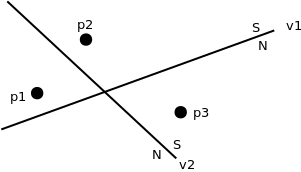
\includegraphics[scale=0.7]{figs/votacao-perfeita.png}
  \caption{Mapa espacial de votação com classificação perfeita.}
  \label{fig:mapa-classificacao-perfeita}
\end{figure}

No exemplo fornecido, podemos ver pelo mapa que o parlamentar $p1$ votou \yea na votação $v1$ e \nay para a votação $v2$. Já $p2$ votou \yea para $v1$ e \yea para $v2$. Por fim, $p3$ votou \nay para $v1$ e \yea para $v2$. Como a partir do mapa descrevemos perfeitamente o comportamento dos parlamentares, dizemos que trata-se de uma votação perfeita.

Mas conforme o número de votações e de parlamentares cresce, percebe-se que é impossível posicionar perfeitamente todos os pontos em relação a todas as retas. Por isso é importante entender que o mapa de votações não é construído de forma a descrever perfeitamente o comportamento dos parlamentares. Em vez disso, o mapa de votações tenta maximizar a quantidade de classificações corretas. 

Na concepção dos trabalhos de Poole, considera-se que em um mapa de votações cada parlamentar possui seu \emph{ponto ideal} no espaço. Nesse mesmo espaço, uma votação também possui pontos associados às suas possíveis opções (\yea e \nay). A reta que representa a votação na Figura~\ref{fig:mapa-classificacao-perfeita} é construída em função desses pontos que representam a votação. Dessa forma, o comportamento de um parlamentar numa dada votação é função de relações entre seu ponto ideal e a representação espacial da votação. 

Dados os pontos ideias associados a parlamentares e votações, uma primeira abordagem simplista para determinar o voto do parlamentar em uma votação seria dizer que o parlamentar vota deterministicamente na opção mais próxima de seu ponto ideal. Mas em vez disso, Poole utiliza o conceito de \emph{função utilidade}, que atribui a cada ponto no espaço um valor. Quanto mais alto esse valor, maior é a \emph{probabilidade} de que o parlamentar vote na opção associada a esse ponto do espaço. 

Duas premissas importantes são usualmente aplicadas às funções utilidade: 1) as funções são de pico único (i.e., possuem apenas um ponto de valor máximo), sendo esse pico localizado no ponto ideal do parlamentar; 2) a função é simétrica, ou seja, o parlamentar é indiferente a duas opções igualmente distantes de seu ponto ideal.

\todo{Fazer figura ilustrativa?}

A função utilidade possui uma parcela determinística e também uma parcela estocástica, que possibilita a modelagem de \emph{erros de votação}. Um erro de votação seria a ideia de que o parlamentar não votou de acordo com suas preferências políticas. Um erro pode ter acontecido no sentido de que o parlamentar pode ter avaliado erroneamente a localização espacial das opções de uma dada votação. Mas o erro pode refletir também o fato de que fatores subjacentes não captados pelo modelo foram decisivos na determinação da opção escolhida.

Dados os conceitos básicos apresentados (pontos ideias, funções utilidade etc.) vamos descrever agora os principais métodos de construção de mapas espaciais de votações elaborados por Poole. São eles o \emph{Optimal Classification} e o NOMINATE.

O \emph{Optimal Classification} (OC) consiste em um processo iterativo\footnote{Um processo iterativo é aquele no qual um algoritmo é repetido várias vezes, sendo que depois de uma certa quantidade de repetições há uma \emph{convergência}, ou seja, o resultado não mais se altera com mais repetições do processo.} que procura maximizar a proporção de classificações corretas em um mapa espacial de votações. Dada uma configuração inicial de um mapa de votações, primeiramente aplica-se um algoritmo que maximiza a classificação correta fixando os pontos e movendo os linhas. Em um segundo passo, fixa-se as linhas e move-se os pontos para maximizar a classificação correta. Esses dois passos são repetidos várias vezes até que o erro (proporção de classificações incorretas) estabilize. Os algoritmos empregados garantem que a cada passo o erro nunca aumenta. 

O OC não define uma posição exata dos parlamentares no mapa de votações, assim como não define uma distância exata entre dois dados parlamentares. O que o OC fornece são regiões do espaço nas quais os parlamentares podem ser posicionados. Essas regiões são denominadas de politopos e representam padrões de opções escolhidas nas votações. Voltemos à Figura~\ref{fig:mapa-classificacao-perfeita}: note que se alterarmos ligeiramente a posição de um parlamentar, digamos $p1$, seu padrão de opções escolhidas não se altera. Esse padrão se mantêm enquanto o ponto ideal não atravessar uma das retas que representam as votações. Dessa forma, dizemos que essa região do espaço delimitada pelas retas que mantêm o padrão de escolhas de $p1$ é o seu politopo.

Após a construção do mapa podemos observar que normalmente alguns parlamentares caem do lado errado de algumas retas. Isso significa que se o leitor do mapa fosse reconstituir os votos dados pelos parlamentares em cada votação, ele se enganaria em alguns casos. Esses erros representam uma imperfeição do mapa construído. A literatura costuma apresentar esses erros como uma incapacidade do modelo obtido em \emph{predizer} corretamente os resultados de algumas votações. É preciso ficar atento com o uso do termo \emph{predição}, pois os mapas de votações ou funções utilidades obtidos não serão utilizados na tentativa de predizer o resultado de votações futuras, ou mesmo votações passadas que não foram utilizadas para a produção do mapa de votações. 

Para a utilização do OC, não é preciso premissas sobre a distribuição da função utilidade. Apenas considerar que ela é simétrica e de pico-único. Embora o conceito de função utilidade não apareça diretamente na aplicação do algoritmo, ele é importante para explicar os erros de classificação, no sentido de que há uma certa probabilidade de que o legislador vote na opção contrária do que o mapa de votações indica.

Como exemplo de aplicação, Poole~\cite{poole2005book} mostra os resultados do OC quando aplicado à votação de revogação das leis do milho na Casa dos Comuns do parlamento inglês em 1846. Nessa situação, o algoritmo apresentou uma taxa de classificação correta de 95,2\% para os 430 parlamentares que votaram nessa matéria. Já em outro estudo mais extenso~\cite{poole-rosenthal2000}, analisando da 80ª à 104ª legislatura do senado dos EUA, Poole obteve taxas de classificação correta para duas dimensões que vão de 85,8\% a 91,3\%.

O outro método de construção de mapas espaciais de votações consagrado por Poole é o \nominate, que constitui na verdade uma família de algoritmos com ligeiras variações entre si. Diferentemente do OC, o \nominate produz posições exatas dos pontos ideais de parlamentares e votações, podendo-se assim atribuir distâncias entre esses pontos. Já o OC produz apenas a localização dos pontos ideias dos parlamentares nos politopos representando padrões de votações.

No \nominate temos algumas premissas a mais sobre as funções utilidade. A mais importante é de que a função utilidade é exponencial. Outra opção utilizada em outros trabalhos~\cite{clinton2004ideal} são funções quadráticas. Essa diferença diz respeito a como o parlamentar vai se comportar em relação a opções cada vez mais longes de seu ponto ideal. Com funções exponencias, as opção cada vez mais longe se tornam cada vez mais indistinguíveis, enquanto que na exponencial elas se tornam cada vez pior avaliadas.

\todo{Fazer figura ilustrativa de função exponencial vs função quadrática.}

Agora vamos detalhar a função utilidade utilizada no \nominate~\cite{poole1985nominate}. Considere a localização $x$ de um parlamentar e a localização $o$ de uma opção de uma votação. Essas localizações são pontos em um espaço multi-dimensional, onde cada dimensão representa preferências sobre um determinado tema político. Para uma votação temos $o_y$, a localização da opção \yea, e $o_n$, a localização da opção \nay. 

A função utilidade utilizada pelo \nominate~\cite{poole1985nominate} é 

\[ U(x,o) = \beta * e^{\frac{-w^2*d^2}{2}} + \varepsilon,\] 

\noindent
onde $d$ representa a distância entre os pontos $x$ e $o$, dada por $|x -o|$. Quanto mais perto $z$ está de $o$, maior o valor de $U$, sendo $U$ simétrica e de pico único. $\beta$ e $w$ são parâmetros da função utilidade, sendo $\beta$ o fator de ruído, que determina o peso da parcela determinística da função utilidade. $\varepsilon$ é a parcela estocástica, que representa erros distribuídos independentemente de conforme a distribuição logística. Poole afirma que teoricamente a distribuição normal para $\varepsilon$ seria mais adequada. No entanto, devido às limitações computacionais da época, Poole optou pela distribuição logística, que é mais simples do ponto de vista computacional e razoavelmente similar à função normal.

No \nominate temos então três grupos de parâmetros: pontos ideias dos parlamentares (um $x$ para cada parlamentar), pontos ideais das opções das votações envolvidas (um $o_n$ e um $o_y$ para cada votação) e os parâmetros da função utilidade ($\beta$ e $w$). O objetivo do \nominate é encontrar os valores de todos esses parâmetros para que se possa desenhar o mapa espacial de votações.

Dada uma configuração inicial de pontos ideias de legisladores e opções de votações, o \nominate aplica sucessivamente os três seguintes passos: 1) estima-se os parâmetros da função utilidade com base nos parâmetros dos legisladores e das votações; 2) estima-se os parâmetros dos legisladores com base nos parâmetros das votações e da função utilidade; 3) estima-se os parâmetros das votações com base nos parâmetros dos legisladores e da função utilidade. Cada um desses passos possui seu próprio algoritmo com suas complexidades. Os três passos são repetidos até a convergência, que é quando o refinamento para de ter efeito e os mesmos valores são produzidos.

Tanto o OC quanto o \nominate partem de uma \emph{configuração inicial} do mapa de votações a ser refinada. Poole define essa configuração inicial pelo seguinte processo: 1) constrói-se uma matriz de concordância entre parlamentares; 2) transforma-se os valores de concordância em distâncias quadráticas; 3) centraliza-se duplamente a matriz de distâncias quadráticas; 4) realiza-se sobre essa matriz uma decomposição de autovetores-autovalores. \Leo{O que comentar sobre esse processo maluco? Alguma relação com o PCA?}

% Texto original do parágrafo acima:
%The best method I have found to get good starting values for the legisla-
%tors is to (1) compute the legislator-by-legislator matrix of agreement scores,
%(2) transform the agreement score matrix into squared distances, (3) double-
%center the matrix of squared distances, and (4) perform an eigenvalue–
%eigenvector decomposition of the double-centered matrix.

Analisando 172 votações realizadas por 440 parlamentares na 85ª legislatura do congresso dos EUA, Poole~\cite{poole1985nominate} obtém uma taxa de classificação correta de 78,9\% utilizando o \nominate com apenas uma dimensão.

\subsection*{Formas de se avaliar os resultados produzidos}

Para avaliar os resultados de um modelo espacial de votações podemos usar a taxa de classificação correta, que nos informa a porcentagem de acertos e erros do modelo. Sendo $U$ a função utilidade, se os parâmetros obtidos pelo modelo definem que $U(\textrm{SIM}) > U(\textrm{NÃO})$ pra um determinado parlamentar em uma determinada votação, temos um acerto caso o parlamentar realmente tenha votado \yea naquela votação ou um erro se na realidade o parlamentar votou \nay.

No entanto, o problema é que modelos extremamente ingênuos podem obter boas taxas de classificação correta. Exemplo: o modelo pode prever que todos os parlamentares votam na opção vencedora. Dessa forma, numa votação em que 90\% dos legisladores votaram com a maioria, o modelo ingênuo teria apenas 10\% de erro. Por isso, utiliza-se também a PRE (redução proporcional do erro)~\cite{leoni02cdep}, que mede em quantos porcentos o erro foi reduzido do modelo ingênuo para o modelo avaliado. Ou seja,

\[PRE = \frac{\textrm{votos da minoria} * \textrm{erros do modelo}}{\textrm{votos da minoria}}.\]

A fórmula da PRE considera apenas uma votação. Para se avaliar um conjunto de votações, se utiliza a APRE (redução proporcional do erro agregado)~\cite{leoni02cdep}, onde a quantidade de votos na minoria e a quantidade de erros são consideradas para todas as votações.

\subsection*{Aplicações no congresso brasileiro}

Aplicando o \wnominate, uma das variações do \nominate, à Câmara dos Deputados, Leoni~\cite{leoni02cdep} encontra taxas de classificação correta de 86,4\% e 90,4\% para as 49ª e 50ª legislaturas respectivamente. Já em termos de APRE, as taxas encontradas são de 52,3\% e 64,8\% para as mesmas legislaturas.

Izumi~\cite{izumi2016senado} elabora mapas espaciais de votações para o Senado brasileiro. No entanto, ele argumenta que o \nominate pode não ser adequado por causa dos pressupostos envolvendo a função utilidade. O primeiro pressuposto questionado é a simetria da função utilidade, uma vez que, por exemplo, a redução em 5\% dos impostos pode ser algo muito mais importante para um parlamentar do que um aumento da mesma magnitude.

O segundo pressuposto questionado da função utilidade é o de que os erros são independentes e identicamente distribuídos entre os legisladores e as votações. Argumentos contrários a esse pressuposto: 1) existem partidos mais coesos que outros (o PT, por exemplo, costuma ser bem mais coeso que outros partidos); 2) migrações de parlamentares entre partidos e migrações de partidos para dentro ou fora da base governista podem alterar a variação de erros ao longo do tempo;  3) em determinados contextos o voto estratégico pode prevalecer sobre o voto sincero. Interessante notar aqui como os argumentos 1) e 2) são características que diferenciam o estudo do legislativo brasileiro do legislativo norte-americano.

Embasado por esses questionamentos, Izumi prefere adotar o Optimal Classification, pois este não se sustenta sobre pressupostos da função utilidade ou da distribuição de erros. Dessa forma, aplicando o OC a seis legislaturas do Senado (48ª a 53ª), Izumi encontra taxas de classificação correta entre 90,7\% e 98,5\%. Já em termos de APRE, as taxas encontradas são entre 50\% e 94\%. Embora o trabalho de Izumi se aplique ao Senado, cabe notar aqui que todos seus argumentos também se aplicariam à Câmara dos Deputados.

Cabe notar que parte das críticas de Izumi ao \nominate se aplicam também ao OC. Como disse Poole~\cite{poole2000oc}, as únicas premissas para a aplicação do OC são 1) o espaço de escolha é euclideano; e 2) preferências são simétricas e de pico-único. Como o próprio Izumi disse, a simetria é uma premissa que pode ser questionada na prática, e essa não somente para o caso brasileiro.

\Leo{Com as considerações do Izumi, talvez não seja mais tão interessante comparar o PCA com o nominate... será q faz sentido comparar com o OC?}

\subsection*{Modelos lineares de Heckman e Snyder}

Muitos trabalhos consideram modelos lineares para a análise de votações nominais menos adequados do que os modelos não lineares, como o \nominate de Poole. Heckman e Snyder~\cite{heckman-snyder1997}, porém, demonstram rigorosamente a equivalência de modelos lineares com os resultados obtidos por Poole, tendo como principal vantagem a simplicidade e eficiência computacional dos métodos lineares.

Para Heckman e Snyder, a decisão de se votar \yea ou \nay em uma votação é modelada como o resultado de um processo de escolha racional no qual os legisladores usam suas preferências para ponderar sobre as características da votação. Assim, dizemos que uma opção é localizada em um espaço no qual cada dimensão seria uma característica da opção. Nesse caso, a função de utilidade recebe um vetor no espaço de características e retorna um número real. Cada legislador teria sua própria função utilidade e escolheria a opção que resultasse no maior valor da função utilidade. Diferentemente do NOMINATE, temos aqui uma função utilidade quadrática.

A função utilidade de Heckman e Snyder, assim como a do NOMINATE, é incrementada com uma parcela de erros aleatórios. Considera-se que uma das fontes de erro seja a dificuldade para o parlamentar estimar o valor de cada característica. 

Os autores utilizam diferentes métodos algébricos para estimar as preferências dos legisladores. Um dos métodos mais simples utilizados é justamente a Análise de Componentes Principais (ACP). \Leo{Elaborar relação entre o PCA e a função utilidade. No que o nosso uso aparentemente mais simples da PCA é diferente do uso aparentemente mais elaborado da PCA como feito por Heckman?}

\subsection*{Dimensionalidade dos mapas de votações}

Um debate existente na literatura é sobre a quantidade de dimensões necessárias para representar um mapa espacial de votações. De acordo com McCarty~\cite{mccarty2011measuring}, essa é uma polêmica sem conclusão definitiva.

Segundo McCarty~\cite{mccarty2011measuring}, a utilização de uma segunda dimensão no D-NOMINATE\footnote{O D-NOMINATE, ou \emph{dynamic \nominate}, é uma variação do \nominate para a comparação intertemporal dos pontos ideais nos mapas de votações.} acrescenta um poder explicativo de apenas 4\% sobre o poder de explicação de 87\% já fornecido pela primeira dimensão. No entanto, de 1945 até a década de 60, questões raciais e de direitos civis fazem com que a segunda dimensão seja mais significativa. 

A primeira dimensão presente nos mapas de votações do legislativo americano estaria ligada ao espectro político-ideológico presente nesse país, possuindo uma escala que vai do extremo liberal ao extremo conservador. No período em que a segunda dimensão se torna significativa, evidencia-se também um padrão de votação que diferencia parlamentares do norte e do sul dos~EUA.  

Já para Heckman e Snyder~\cite{heckman-snyder1997}, existem pelo menos cinco dimensões significativas. Essas dimensões a mais podem não fazer tanta diferença na taxa global de sucesso de classificação, mas são decisivas em algumas votações específicas, por representarem substantivamente assuntos específicos. Exemplos de tais assuntos: direitos civis e eleitorais, agricultura, ajuda internacional, gasto militar, teto da dívida, água, aborto e reforma do congresso.

Utilizando o W-NOMINATE, Leoni~\cite{leoni02cdep} chegou à conclusão de que uma dimensão explica a maior parte das votações na Câmara dos Deputados, pois dimensões adicionais não melhoram significativamente a capacidade explicativa do modelo.

% leoni traduz "outcome" como "consequência política"

\subsection*{Discussão}

\Leo{Oi Saulo, principalmente essa parte que eu queria ver oq vc acha... se oq tá escrito aí não é besteira =S}

Como visto, os trabalhos em ciências políticas normalmente não buscam somente a elaboração de mapas espaciais de votações, mas também a elaboração de teorias e modelos que embasem esses mapas. Porém, toda teoria parte de algumas suposições, que no caso concreto podem ou não serem verdadeiras. Davis et al.~\cite{davis1970electoral}, por exemplo, pressupõe que todos os eleitores avaliam os candidatos sob o prisma dos mesmo assuntos. Poole, tanto no OC quanto no \nominate, pressupõe funções utilidade simétricas e de pico único. Já no \nominate, temos ainda que considerar que erros são independentes e identicamente distribuídos. Mesmo Heckman e Snyder~\cite{heckman-snyder1997}, que utilizam modelos lineares, se apoiam fortemente em modelos de escolha discretas, considerando que o legislador modela suas preferências de forma multidimensional e aplica uma função utilidade quadrática sobre esses valores para tomar sua decisão.

Embora o uso de suposições para a elaboração de teorias seja comum e necessário, podemos aqui ponderar sobre uma vantagem da utilização da ACP para a elaboração dos mapas de votações. Como trata-se de uma abordagem puramente algébrica, sem uma teoria por trás, podemos entender o gráfico gerado pela ACP como uma fotografia do comportamento dos parlamentares em um determinado período. Essa fotografia não é perfeita, há uma perda de informação, mas que pode ser medida como veremos mais a frente. Essa fotografia não traz consigo explicações sobre o processo de decisão ou do porquê dos resultados, mas possibilita a um analista político que faça considerações sobre a conjuntura política de uma determinada casa legislativa em um determinado período, ajudando o analista a chegar a possíveis conclusões.

Ou seja, mesmo sem o embasamento de uma teoria, o mapa de votações produzido pela ACP é útil. E justamente por não estar baseado em uma teoria forte, pode-se dizer que esse mapa não tem a validade limitada por suposições que podem não ser verdadeiras no caso concreto.




\section{Decisões de nossa abordagem}

Dizer que utilizamos o PCA e como modelamos nossa matriz de entrada conta apenas parte da história. Ao utilizar o PCA diversas outras pequenas decisões devem ser feitas. Nesta seção tratamos dessas decisões, assim como algumas variações do tipo de análise. Algumas dessas decisões são feitas em função das características do sistema político brasileiro, em contraste com o sistema político do EUA, usalmente abordado na literatura.

\subsection*{Análise por partido}

No modelo apresentado, nada impede que os valores de $\mathbf{X}$ possuam valores reais, situados por exemplo no intervalo [-1;1], em vez de apenas os valores discretos \{-1;0;1\}. Esta observação permite uma extensão direta do modelo para analisar os parlamentares agregados por partido em vez de considerá-los individualmente, bastando considerar o voto médio do partido em cada votação antes de iniciar a análise.

O voto médio do partido $k$ na votação $i$ é definido por:
\begin{equation}
  x_{ik} = \frac{1}{|k|}\sum_{j\in k} x_{ij}
  \label{eq:voto-partido}
\end{equation}
onde $j \in k$ denota que o parlamentar $j$ pertence ao partido $k$, e $|k|$ é o número de parlamentares do partido $k$ considerados.

Esta análise é útil para analisar afinidades partidárias e coalizões em ambientes com vários partidos, como é tipicamente o caso das casas legislativas no Brasil.

\ins{No Radar Parlamentar, porém, não aplicamos essa técnica, pois para esse software optamos pela coexistência de partidos e parlamentares individuais no mesmo mapa especial. O método proposto acima é válido, mas seu resultado não possui relação direta com o resultado da análise por parlamentar. Assim sendo, no Radar Parlamentar os partidos são posicionados no centroide das posições ocupadas por seus parlamentares. Segue fórmula da hora...}

\subsection*{Tratamento de valores faltantes}

Todos os métodos de análise de votações legislativas encontrados na literatura revisada descartam ausências e abstenções antes de iniciar a análise, considerando explicita- ou implicitamente que tais atitudes não trazem informação acerca das preferências políticas do legislador, e notando que tais situações representam a minoria dos casos. Por exemplo, Heckman e Snyder notam que as abstenções representam menos de 1\% dos votos para câmara e senado estadounidenses, e as assumem aleatórias em relação a resultados das votações e a preferências dos parlamentares \cite[p.40]{heckman-snyder1997}.

Já 53a legislatura da Câmara dos Deputados brasileira (período de 2003 a 2006) soma para votações nominais abertas cerca de 6\% entre abstenções e obstruções, e as ausências são próximas de 49\%. Propõe-se que o comportamento observado de ausentar-se ou abster-se de uma votação traz sim informação acerca das preferências do parlamentar que se deseja estimar, e por isso essa informação não deve ser descartada na análise.

No modelo proposto, ausência, abstenção e obstrução são modeladas através do valor 0. Em relação à alternativa de descartar estas situações, que serão referidas genericamente como votos ``nulos'', esta modelagem introduz um viés no sentido oposto ao voto médio dos que realmente votaram. Ou seja, supondo sem perda de generalidade que o voto da maioria é sempre SIM, o voto médio dos que votaram será sempre maior que zero, e se o parlamentar faz voto nulo sua preferência nesta votação será modelada como sendo ligeiramente oposta ao SIM (pois seu voto é numericamente menor do que a média), mas não tão oposta quanto se o parlamentar tivesse efetivamente votado NÃO.

Este viés pode parecer arbitrário, porém esta abordagem é consistente tanto com a idéia de que um voto nulo representaria uma indiferença do parlamentar quanto aos resultados SIM e NÃO (o voto nulo é euclidianamente equidistante das duas alternativas) quanto da idéia de que ao não votar o parlamentar pode ter uma preferência contrária àquela que se imagina que será aprovada na votação, como em um ``boicote'' pessoal (ou em grupo) à votação. Em outras palavras, um parlamentar teria maior tendência de comparecer e não se abster nem obstruir a votação em propostas nas quais ele esteja inclinado a votar com a maioria. Se estas hipóteses são arbitrárias, pode-se dizer que são pelo menos tão arbitrárias quanto a alternativa de considerar que um voto nulo equivale a um parlamentar com preferência igual à preferência média da casa. Nossos resultados sugerem que de fato a forma proposta de modelagem melhora os índices de classificação correta.

No caso da análise por partidos, ao excluir votos nulos do cálculo da média na equação \ref{eq:voto-partido} estaria-se buscando considerar que a opinião ``do partido'' é composta apenas pela opinião daqueles que votaram ou SIM ou NÃO. Outra opção é excluir apenas as ausências, se os dados permitirem discriminar esta opção. Os resultados aqui apresentados não excluem estes votos, para que a análise reflita o fato de que uma abstenção ou mesmo uma ausência não são equivalentes a concordar com a opinião geral do partido. Além disso a análise fica mais simples, já que não há necessidade de tratamento especial de partidos que tenham estado por exemplo cem porcento ausentes em uma dada votação.

\subsection*{Tratamento de votações unânimes}

E tb de parlamentares que faltam bastante.

Acho que no caso, simplesmente não consideramos esses problemas e usamos todo mundo.

Mas pelo menos sobre votações unânimes isso tem a parte ruim de deixar o mapa mais embolado e difícil de ler. Por outro lado, ajuda a mostrar a realidade de que na prática, apesar das diferenças, eles não são tão diferentes assim.

\nominate faz uns cortes pra não pegar todo mundo.

\subsection*{Lidando com migração partidária}

Citar Izumi

\subsection*{Análise temporal}

O objetivo de nossa análise temporal não é que se possa comparar as posições de um parlamentar/partido ao longo do tempo, mas que se possa comparar as distâncias relativas desses elementos entre si ao longo do tempo.

Efeito de extremistas na visualização temporal: um extremista de um período afeta a visualização de outros períodos (deixando parlamentares muito concentrados). Procede ???

\Leo{Comparar em linhas gerais nosso método de análise temporal com o D-NOMINATE (dynamic nominate).}


Heckman encontra uma alta correção entre as coordenadas de um legislador ao longo do tempo (e não são apenas para as duas primeiras coordenadas... chega-se a até 6 ou 8 fatores com correlação ao longo do tempo). Mas duvido que no caso brasileiro essas correlações seriam altas.

\subsection*{Quantidade de dimensões utilizadas}

Quantidade defina a priori, pois duas dimensões pode-se visualizar facilmente no plano. Se segunda dimensão explica pouca coisa a mais, tudo bem, isso ficará evidente pela dispersão dos pontos no gráfico.

\section{Medidas de Adequação (Fitness)}
\label{sec:metodo}

\ins{Aqui, explicar os indicadores e tal.}

\section{Resultados}
\label{sec:resultados}

\ins{Mostrar resultados de indicadores e gráficos.}

As análises foram feitas no software de estatística \textbf{R} \footnote{O código dos scripts utilizado está disponível em \url{https://github.com/leonardofl/radar_parlamentar} sob licensa \emph{AGPL v3}} Como referência para \emph{benchmarking} foi adotado o algoritmo WNOMINATE, através do pacote \emph{wnominate} para \textbf{R} \footnote{O pacote wnominate pode ser encontrado na \emph{Comprehensive R Archive Network}, no endereço  \url{http://CRAN.R-project.org/package=wnominate}}.

...

Heckman e Snyder~\cite{heckman-snyder1997} encontram padrões políticos na distribuição do mapa espacial que são compatíveis com análises já feitas por cientistas políticos utilizando outros métodos. These findindgs illustrate the ``reasonableness'' of estimates obtained from our model. Vamos na mesma linha... mostrar que nossos mapas obtidos fazem sentido do ponto de vista político.

...

Problema da taxa de classificação correta no PCA: para modelar as votações, mapeando opções em valores numéricos, tudo bem. Mas o cálculo da taxa de classificação correta depende do mapeamento inverso, dado um valor entre -1 e 1 definir uma das opções (\yea, \nay ou ABSTENÇÃO). Definir os valores limiares desse mapeamento inverso é arbitrário, sendo que essa escolha arbitrária pode alterar drasticamente os valores obtidos. 

Em vez de se valer da taxa de correta classificação, uma medida melhor para avaliar o resultado do mapa espacial gerada pela ACP é o porcentual da variância dos dados explicados pelas dimensões utilizadas no mapa. No entanto, essa medida tem a desvantagem de não ser diretamente comparável com outros métodos.


\section{Discussão}
\label{sec:discussao}

\ins{Comparar pros e contras dos algoritmos, e contextualizar (ferramenta web, características brasil, vantagens políticas de análise mais transparente e simples etc.)}

\section{Conclusões}
\label{sec:conclusoes}

\ins{resultados
 coisas pra melhorar / investigar
 ex: modelagem de partidos q não votam em alguma votação; suplentes; troca de parlamentares análise de sensibilidade }


\bibliography{refs}{}
\bibliographystyle{ieeetr}
 
\end{document}
